\documentclass[11pt,a4paper]{article}

\usepackage[T1]{fontenc}
\usepackage[utf8]{inputenc}
\usepackage[brazil,english]{babel}
\usepackage{lmodern}
\usepackage{microtype}
\usepackage{geometry}
\geometry{top=2.5cm,bottom=2.5cm,left=2.7cm,right=2.7cm}

\usepackage{amsmath,amssymb}
\usepackage{booktabs,longtable,tabularx,array}
\usepackage{graphicx,float,caption}
\usepackage{xcolor}
\usepackage{enumitem}
\usepackage{needspace}
\usepackage{etoolbox}
\pretocmd{\section}{\Needspace{5\baselineskip}}{}{}
\pretocmd{\subsection}{\Needspace{4\baselineskip}}{}{}
\setlength{\emergencystretch}{2em}
\usepackage[round,authoryear]{natbib}
\usepackage[hidelinks]{hyperref}
\usepackage[nameinlink,noabbrev]{cleveref}

\definecolor{gppmeblue}{HTML}{8A421E}
\definecolor{gppmelight}{HTML}{F3F5F2}
\hypersetup{
  colorlinks=true,
  linkcolor=gppmeblue,
  citecolor=gppmeblue,
  urlcolor=gppmeblue,
  pdflang={pt-BR},
  pdftitle={GEAR: construção de um framework de governança de TI com pesquisa assistida por IA e auditoria de conteúdo},
  pdfauthor={André Victor Andrade Oliveira Santos}
}

\setlength{\parindent}{1.25cm}
\setlength{\parskip}{0.15em}
\renewcommand{\arraystretch}{1.18}
\captionsetup{font=small,labelfont=bf}
\newcolumntype{L}[1]{>{\raggedright\arraybackslash}p{#1}}
\newcolumntype{R}{>{\raggedright\arraybackslash}X}

\title{\textbf{GEAR: construção de um framework de governança de TI para pequenas empresas com pesquisa assistida por IA e auditoria de conteúdo}}
\author{Andr\'{e} Victor Andrade Oliveira Santos\\
Instituto Federal de Educa\c{c}\~{a}o, Ci\^{e}ncia e Tecnologia da Bahia (IFBA)\\
Campus Vit\'{o}ria da Conquista}
\date{Primeira versão: agosto de 2026. Revisão editorial: outubro de 2026}

\begin{document}
\selectlanguage{brazil}
\maketitle

\begin{center}
\fcolorbox{gppmeblue}{gppmelight}{%
  \parbox{0.91\textwidth}{\small\textbf{Nota de versão.}
  Este manuscrito apresenta a construção do GEAR e o uso de IA com auditoria de conteúdo durante a produção. A prova de conceito no FrameSim é futura: os 25 casos comparativos ainda não foram executados e não há resultados de validação do framework.}}
\end{center}

\begin{abstract}
Este artigo apresenta a construção do GEAR (Gestão, Execução, Agilidade e Risco), um framework de governança e gestão de TI destinado a pequenas empresas com recursos restritos, e documenta o uso ativo de inteligência artificial (IA) na pesquisa e na produção do material. O estudo segue Design Science Research e combina leitura dirigida da literatura, seleção de referências gerenciais, síntese assistida e auditoria de conteúdo. O procedimento distingue afirmações externas, adaptações autorais e hipóteses; verifica fontes, versões, unidades e limites de generalização; e registra correções sob responsabilidade autoral. O artefato resultante organiza três domínios essenciais, um percurso inicial de 30 dias, modelos compactos e indicadores, com assistência por IA opcional na aplicação. A evidência disponível permite inspecionar o desenho e a rastreabilidade documental, mas não medir o ganho causado pela IA nem a efetividade organizacional do GEAR. Sua avaliação será uma prova de conceito futura no FrameSim, com 25 empresas sintéticas de 5 a 20 colaboradores, comparações pareadas com ITIL~4 e COBIT~2019 adaptados e critérios de análise previamente definidos. Nenhuma rodada de cenários foi executada para esta versão. As contribuições atuais são a especificação do framework, o relato da produção assistida com auditoria de conteúdo e o protocolo prospectivo de avaliação.

\noindent\textbf{Palavras-chave:} governança de TI; pequenas empresas; teoria da contingência; Design Science Research; inteligência artificial; simulação baseada em personas.
\end{abstract}

\clearpage
\begin{otherlanguage}{english}
\begin{abstract}
This paper presents the construction of GEAR, an IT governance and management framework for small firms with limited resources, and documents the active use of artificial intelligence (AI) in research and content production. Following Design Science Research, the study combines directed literature reading, selection of management references, assisted synthesis, and content auditing. The procedure distinguishes external claims, authorial adaptations, and hypotheses; checks sources, versions, units, and generalization limits; and records corrections under authorial responsibility. The resulting artifact comprises three essential domains, a 30-day adoption route, compact templates, and indicators, with optional AI assistance during application. Available evidence supports inspection of the design and documentary traceability, but does not measure the causal benefit of AI or GEAR's organizational effectiveness. Evaluation will take the form of a future proof of concept in FrameSim, using 25 synthetic firms employing 5 to 20 people, paired comparisons with tailored ITIL~4 and COBIT~2019, and predefined analysis criteria. No scenario runs were conducted for this version. Current contributions are the framework specification, an account of assisted production with content auditing, and a prospective evaluation protocol.

\noindent\textbf{Keywords:} IT governance; small firms; contingency theory; Design Science Research; artificial intelligence; persona-based simulation.
\end{abstract}
\end{otherlanguage}

\section{Introdução}
\label{sec:introducao}

A tecnologia da informação tornou-se parte do funcionamento cotidiano de empresas pequenas: sustenta vendas, atendimento, faturamento, comunicação e continuidade operacional. Para organizações com equipes reduzidas, entretanto, governar essa dependência cria um problema prático. As decisões de TI costumam se concentrar no proprietário e em um profissional interno ou terceirizado, enquanto orçamento, tempo e especialização permanecem limitados. Nesse contexto, a ausência de governança aumenta a exposição a prioridades conflitantes, interrupções e riscos; a adoção literal de estruturas extensas, por outro lado, pode introduzir um custo de coordenação incompatível com a capacidade da organização.

O problema não decorre da falta de referências consolidadas. A ISO/IEC~38500 orienta o corpo governante a avaliar, direcionar e monitorar o uso da TI \citep{iso38500_2024}; o COBIT~2019 oferece componentes e fatores de desenho para sistemas de governança \citep{isaca2018cobit}; o ITIL~4 organiza a gestão de produtos e serviços em torno da criação de valor \citep{axelos2019itil}; e o NIST CSF~2.0 e os CIS Controls~v8 estruturam a gestão de riscos de segurança \citep{nist2024csf,cis2021controls}. O desafio está em transformar esse corpo de conhecimento em um conjunto mínimo, coerente e executável por uma empresa com poucas pessoas, sem descaracterizar os princípios que lhe dão sustentação.

A literatura oferece suporte para uma abordagem contingencial. \citet{levstek2022adaptive} observam que mecanismos de governança de TI não são universalmente necessários e que modelos abrangentes podem ser onerosos para pequenas e médias empresas. Em uma linha complementar, \citet{silva2018baseline} identificam mecanismos estruturais, processuais e relacionais que podem formar uma base mínima de governança, embora seu estudo exploratório tenha uma amostra reduzida. A revisão sistemática de \citet{sagala2024transformation} reforça que a transformação digital em PMEs deve considerar a situação inicial, as limitações e as idiossincrasias da organização, com implantação incremental e aprendizagem contínua. Essas evidências apontam para a necessidade de seleção e adaptação, e não para a simples redução de um único framework.

Este trabalho responde à seguinte questão de pesquisa: \emph{como estruturar um artefato de governança e gestão de TI que preserve mecanismos essenciais de direção, execução e segurança, mas seja operável por empresas com recursos humanos e financeiros restritos?} Como delimitação empírica futura, o estudo concentra sua primeira avaliação em empresas simuladas com 5 a 20 colaboradores. Esse recorte corresponde ao ambiente organizacional para o qual o custo de coordenação e a concentração de papéis tendem a ser mais críticos; ele não autoriza generalizações para todo o universo estatístico das PMEs.

Propõe-se o GEAR (Gestão, Execução, Agilidade e Risco), um artefato contingencial composto por três domínios essenciais: governança e direção, execução e serviços, segurança e continuidade. Uma camada transversal e opcional de assistência por inteligência artificial (IA) apoia diagnóstico, documentação, métricas e consulta ao conhecimento do framework, sempre com revisão humana. A adoção começa por um percurso local de 30 dias, historicamente chamado Fase Zero, destinado a criar visibilidade sobre demandas, decisões, ativos, riscos e indicadores. O prazo orienta o planejamento e não garante implantação ou avanço de maturidade.

O GEAR é apresentado como uma síntese de desenho, não como substituto normativo para ISO/IEC~38500, COBIT, ITIL, NIST CSF ou CIS Controls. O artefato seleciona mecanismos compatíveis com seu contexto-alvo e mantém rastreabilidade até as referências de origem. Essa distinção é especialmente importante na comparação planejada: COBIT trata de governança e gestão empresarial de informação e tecnologia, enquanto ITIL enfatiza gestão de produtos e serviços. Portanto, a avaliação não buscará declarar um vencedor universal, mas examinar o ajuste entre escopo, esforço de adoção e utilidade produzida em um conjunto controlado de tarefas.

A construção do GEAR também coloca uma questão de método: como usar IA na pesquisa, síntese e produção de documentação sem transformar conteúdo gerado em evidência? Este artigo relata o uso ativo dessa assistência com auditoria de fontes, consistência e cálculos, distinguindo a produção do material da aplicação futura do framework. A contribuição é descritiva e rastreável; não se estima um ganho de produtividade da IA nem se presume que a revisão elimine todos os erros.

As contribuições desta etapa são a especificação de um framework ajustável ao contexto de pequenas equipes, o relato da pesquisa e produção assistidas por IA com auditoria de conteúdo e um protocolo para prova de conceito futura. Os 25 casos comparativos da \cref{sec:protocolo} serão executados no FrameSim após o congelamento de cenários e critérios. Tabelas e figuras de resultados permanecem sem valores. Recursos agregados, como MCPs, skills e integrações, são citados como canais associados ao repositório; sua implementação não integra a contribuição ou a validação deste artigo.

O restante do artigo apresenta a literatura e as bases gerenciais na \cref{sec:fundamentacao}, a pesquisa e a auditoria de conteúdo na \cref{sec:metodo}, e a especificação do GEAR na \cref{sec:artefato}. As \cref{sec:estado,sec:protocolo} distinguem o estado documental e a prova de conceito futura. As \cref{sec:discussao,sec:conclusao} discutem o alcance das contribuições e os limites da evidência.

\section{Fundamentação e trabalhos relacionados}
\label{sec:fundamentacao}

\subsection{Governança adaptativa em organizações pequenas}

A governança de TI pode ser operacionalizada por estruturas, processos e mecanismos relacionais que definem direitos decisórios, coordenam negócio e tecnologia e monitoram a geração de valor. Em organizações pequenas, a utilidade desses mecanismos depende de fatores contingenciais como porte, centralização, maturidade, setor e disponibilidade de competências. O estudo de caso de \citet{levstek2022adaptive} mostra que uma parcela relevante dos mecanismos analisados é situacional e adverte que modelos universais podem ser custosos e difíceis de aplicar em PMEs. Como se trata de um único caso, o resultado fundamenta o desenho adaptativo, mas não demonstra por si só qual configuração é superior em outros contextos.

O estudo exploratório de \citet{silva2018baseline}, baseado em entrevistas semiestruturadas, investiga mecanismos de linha de base para governança empresarial de TI em PMEs. O registro institucional consultado confirma essa abordagem; o número de participantes e a distribuição detalhada dos mecanismos não foram verificados no texto integral. No GEAR, comunicação entre negócio e TI, acompanhamento de orçamento e responsabilidades são escolhas de desenho explicitadas em rotinas, sem atribuir a esse estudo a validação dessas práticas locais.

A transformação digital acrescenta uma dimensão temporal ao problema. A revisão sistemática de \citet{sagala2024transformation} recomenda que PMEs considerem sua linha de base e suas limitações, com avanços incrementais e investimento contínuo em aprendizagem. Essa orientação sustenta dois requisitos do GEAR: a entrada por uma fase curta de estabilização e o aumento gradual de práticas conforme evidências de maturidade. A revisão também registra concentração geográfica de estudos, o que recomenda cautela ao transferir seus achados para micro e pequenas empresas brasileiras.

\subsection{Bases normativas e gerenciais}

O acervo histórico relaciona o ciclo local de avaliar, dirigir e monitorar à ISO/IEC~38500:2024 \citep{iso38500_2024}. O texto integral da norma não foi verificado nesta revisão; a associação histórica não demonstra conformidade. No GEAR, ADM-Lite nomeia uma adaptação local, distinta do Architecture Development Method do TOGAF. O COBIT~2019 amplia esse domínio ao oferecer objetivos, componentes e fatores de desenho para um sistema de governança ajustado ao contexto \citep{isaca2018cobit}. O GEAR não reproduz o catálogo do COBIT; usa sua orientação a objetivos e desenho como origem para um subconjunto rastreável de decisões, responsabilidades e métricas.

O ITIL~4 oferece a principal referência para execução e entrega de serviços. Seus princípios orientadores, que orientam adoção e adaptação às necessidades específicas, conforme a apresentação pública consultada \citep{peoplecert2026public}, são compatíveis com a proposta de adequação ao contexto. No GEAR, essa orientação é materializada por canal único de demanda, quadro Kanban com limite de trabalho em progresso, ciclos semanais e um PRD de uma a duas páginas para iniciativas que exijam desenvolvimento. Essa seleção não representa uma implementação integral do sistema de valor de serviço do ITIL.

Para segurança, o NIST CSF~2.0 organiza resultados de gestão de risco nas funções Governar, Identificar, Proteger, Detectar, Responder e Recuperar \citep{nist2024csf}. Os CIS Controls~v8 acrescentam salvaguardas priorizadas e grupos de implementação; o IG1 é apresentado como higiene cibernética essencial e reúne 56 salvaguardas \citep{cis2026ig1}. O GEAR usa essas referências para formar uma linha de base centrada em inventário de ativos críticos, identidade e privilégio mínimo, backup verificável e resposta a incidentes. A expressão ``NIST-Lite'' usada no artefato designa uma adaptação interna e não uma publicação ou certificação do NIST.

\begin{table}[htbp]
  \centering
  \caption{Posicionamento das referências e do GEAR. A comparação descreve escopo e mecanismo, não efetividade observada.}
  \label{tab:posicionamento}
  \small
  \begin{tabularx}{\textwidth}{@{}L{2.3cm}L{3.0cm}R R@{}}
    \toprule
    Referência & Escopo predominante & Força aproveitada & Tradução no GEAR \\
    \midrule
    ISO/IEC 38500 & Referência histórica de governança & Texto integral não verificado nesta revisão & Associação histórica ao ADM-Lite, sem alegação de conformidade \\
    COBIT 2019 & Governança e gestão de informação e tecnologia & Objetivos, componentes e fatores de desenho & Rastreabilidade, responsabilidades e portfólio mínimo \\
    ITIL 4 & Gestão de produtos e serviços digitais & Foco em valor, fluxo e melhoria iterativa & Canal único, Kanban, ciclos semanais e PRD curto \\
    NIST CSF 2.0 & Resultados para gestão de risco cibernético & Funções de governança e ciclo de risco & Organização do pilar de Segurança Crítica \\
    CIS Controls v8 & Salvaguardas cibernéticas priorizadas & IG1 e ações mensuráveis de higiene essencial & Checklist mínimo e evidências operacionais \\
    \bottomrule
  \end{tabularx}
\end{table}

\subsection{IA como assistência, não como fonte de verdade}

Há evidência de que sistemas de IA generativa podem elevar produtividade em tarefas delimitadas. No experimento controlado de \citet{peng2023copilot}, 95 desenvolvedores profissionais implementaram um servidor HTTP em JavaScript; o grupo com GitHub Copilot concluiu a tarefa 55,8\% mais rápido, com intervalo de confiança de 95\% entre 21\% e 89\%. Em outro contexto, \citet{brynjolfsson2025work} analisaram a introdução de assistência por IA entre 5.172 agentes de suporte e observaram aumento médio de 15\% nas questões resolvidas por hora, concentrado entre trabalhadores menos experientes. Esses resultados motivam a hipótese de aceleração documental, mas não podem ser transferidos diretamente para governança de TI nem usados como estimativa de ganho do GEAR.

A engenharia de prompts oferece meios para fornecer contexto, restrições e exemplos a modelos sem alterar seus parâmetros \citep{sahoo2025prompt}. Em pesquisa qualitativa, o mapeamento de \citet{barros2025qualitative} identifica potencial de automação, mas também dependência de prompts, imprecisões ocasionais e limitações contextuais. Por isso, o módulo de IA do GEAR exige dados de origem, indicação de lacunas, citações quando aplicáveis e aprovação humana antes que uma saída gere decisão ou ação.

Referências históricas sem fonte primária confirmada foram separadas dos fundamentos desta edição. O registro de revisão bibliográfica conserva as lacunas e as decisões de restrição.

\subsection{Lacuna e distinção do artefato}

Os trabalhos existentes sustentam a adaptação contingencial, os mecanismos mínimos e a implantação incremental, enquanto as normas oferecem cobertura conceitual robusta. Permanece, porém, uma lacuna entre essas orientações e uma implementação integrada que uma equipe muito pequena consiga iniciar, medir e revisar. O GEAR ocupa esse espaço ao combinar três domínios essenciais, uma porta de entrada temporal, artefatos compactos e uma camada opcional de automação com controles de validação.

A novidade reivindicada é de composição e operacionalização, não a criação isolada dos mecanismos de governança, agilidade ou segurança. O valor científico esperado está na justificativa explícita das escolhas, na rastreabilidade entre fonte e prática, e na avaliação do ajuste organizacional sob protocolo comparativo. Essa formulação torna verificável tanto a contribuição quanto seus limites.

\section{Método de pesquisa e produção assistida}
\label{sec:metodo}

\subsection{Estratégia e delimitação}

O estudo adota Design Science Research (DSR) para relacionar o problema organizacional à construção e à avaliação de um artefato \citep{hevner2004design}. As atividades da DSRM organizam identificação do problema, objetivos, desenho, demonstração, avaliação e comunicação \citep{peffers2007dsrm}. Nesta etapa, o trabalho concentra-se na pesquisa de desenho e na produção documental; a avaliação por cenários permanece prospectiva. A organização segundo DSRM não implica que todas as atividades já tenham sido concluídas.

A pesquisa possui dois objetos articulados: a especificação do GEAR e o procedimento de produção dessa especificação com IA e auditoria de conteúdo. O framework é descrito por conceitos, três domínios essenciais, rotinas e modelos de registro. O segundo objeto explicita como materiais de origem foram selecionados, sintetizados, adaptados e corrigidos. A unidade de inspeção documental é a afirmação ou prática e sua relação com a fonte. Na prova de conceito futura, a unidade de comparação será o caso de empresa sintética, mantido constante entre os três frameworks.

\begin{figure}[H]
  \centering
  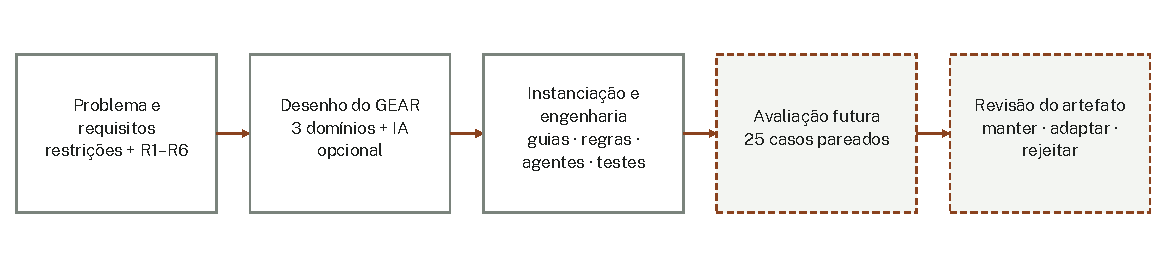
\includegraphics[width=\textwidth]{figures/generated/research-pipeline.pdf}
  \caption{Produção assistida e auditoria de conteúdo nesta etapa; prova de conceito no FrameSim e revisão por resultados em etapas futuras. A IA auxilia a produção, mas não substitui a fonte nem o julgamento autoral.}
  \label{fig:processo-pesquisa}
\end{figure}

\subsection{Leitura dirigida e requisitos de desenho}

A pesquisa partiu do projeto de TCC~I e do acervo histórico GP-PME, com leitura dirigida de estudos sobre governança em PMEs, transformação digital incremental, referências gerenciais e assistência por IA. Trata-se de uma síntese orientada ao desenho, sem protocolo de revisão sistemática exaustiva ou contagem completa de buscas, exclusões e duplicatas. Os estudos e documentos utilizados estão identificados na bibliografia e nas fichas de fontes do núcleo documental. Quando somente uma página institucional, resumo ou apresentação pública pôde ser consultado, o limite de acesso foi registrado; não se pressupõe leitura integral de livros ou normas fechadas.

O desenho adotou seis requisitos: \textbf{R1}, operação por equipe mínima e acumulação explícita de papéis; \textbf{R2}, início incremental; \textbf{R3}, cobertura conjunta de direção, execução e risco; \textbf{R4}, evidência simples por prática; \textbf{R5}, funcionamento integral sem IA; e \textbf{R6}, rastreabilidade e revisão humana quando houver IA. São critérios autorais de desenho, informados pela literatura e pelo contexto-alvo. A sua adequação dependerá da avaliação futura.

\subsection{Uso ativo de IA e auditoria de conteúdo}
\label{sec:auditoria-ia}

A IA participou da produção como instrumento de leitura, síntese e revisão. Foi usada para localizar e organizar trechos do acervo, propor minutas, comparar versões, apontar conflitos terminológicos e apoiar a preparação editorial. A auditoria de conteúdo constitui uma etapa distinta: uma sugestão plausível precisa de fonte ou de identificação explícita como adaptação autoral antes de integrar o material publicado. A assistência também pode propor verificações, mas concordância entre saídas de IA não constitui confirmação independente.

O procedimento de revisão é organizado em seis operações. (1) Identificar a fonte, versão, endereço e limite de acesso. (2) Extrair o conceito e o contexto em que a fonte o sustenta, preservando população, tarefa e período de resultados numéricos. (3) Produzir uma síntese assistida, separando citação, paráfrase e proposta local. (4) Confrontar afirmações com os trechos consultados e conferir unidades, fórmulas e consistência entre documentos. (5) Corrigir, restringir ou excluir conteúdo sem suporte e submeter escolhas à revisão autoral. (6) Registrar a versão, o destino editorial e os limites remanescentes. Essa sequência explicita o procedimento aplicado à revisão atual; não reconstrói um histórico completo de todas as interações anteriores.

A auditoria teve efeitos concretos no conteúdo. Resultados de produtividade obtidos em outras tarefas foram mantidos com seus limites, sem convertê-los em ganho esperado do GEAR. O material financeiro passou a distinguir ROI líquido, razão bruta e capacidade potencial liberada. O questionário de maturidade foi revisto para permitir atingir o nível máximo sem adoção de IA. A nomenclatura passou a fixar três domínios essenciais e assistência opcional. As fichas de origem e o \href{https://github.com/andrecodexvictor/GP-Pme/tree/codex/gear-editorial/framework/publicacao}{registro editorial} permitem examinar essas decisões e localizar suas fontes.

Os registros disponíveis são evidências de processo e de revisão, sem mensuração causal do benefício da IA. Não houve grupo de controle para a produção do material, medição uniforme do tempo de escrita ou avaliação independente de toda afirmação. Parte do histórico não registra de forma uniforme modelo, parâmetros, prompts e intervenções humanas. Esses limites impedem estimar taxa de acerto, redução de esforço ou superioridade da produção assistida. A auditoria reduz incertezas específicas; não garante ausência de erros.

\subsection{Conversão da pesquisa em práticas}

A síntese foi convertida em rotinas com evento de início, responsável, entrada, saída e evidência de encerramento. Cada prática preserva sua finalidade e declara o que foi adaptado ao contexto de equipes pequenas. Os mecanismos são conectados pelo percurso diagnosticar, decidir, executar, verificar e revisar, descrito na \cref{sec:artefato}. Guias, exemplos e modelos permitem inspecionar como a proposta poderia ser aplicada, sem serem resultados de aplicação em empresas.

A demonstração atual é documental: arquitetura, requisitos, guias e instrumentos estão disponíveis para leitura e crítica. Exemplos didáticos expõem premissas e possíveis decisões. A coerência documental e a conferência de cálculos verificam aspectos do artefato, mas não demonstram aprendizagem, adesão ou melhoria organizacional. MCPs, skills e demais integrações do repositório são mencionados como recursos associados e permanecem fora da análise e da validação deste artigo.

\subsection{Mapa de afirmações e evidências}

A \cref{tab:claim-evidence} delimita o que pode ser afirmado nesta etapa. A distinção entre registro de produção, hipótese de desenho e efeito observado orienta a escrita do manuscrito e o protocolo futuro.

\begin{table}[htbp]
  \centering
  \caption{Afirmações centrais, suporte disponível e limites.}
  \label{tab:claim-evidence}
  \small
  \begin{tabularx}{\textwidth}{@{}L{3.0cm}R R@{}}
    \toprule
    Afirmação & Suporte disponível & Limite ou evidência futura \\
    \midrule
    A governança precisa de ajuste ao contexto de PMEs & Estudos e revisão de literatura & Transferência ao recorte brasileiro exige estudo próprio \\
    O GEAR possui uma especificação documental & Núcleo, guias, modelos e fontes versionados & Usabilidade e cobertura precisam de avaliação independente \\
    A produção usou IA e auditoria de conteúdo & Declaração de uso, fontes e registros de revisão & Histórico incompleto; sem medida causal de benefício da IA \\
    O GEAR pode reduzir esforço de coordenação & Hipótese derivada de rotinas e artefatos compactos & Prova de conceito com alternativas comparáveis \\
    O GEAR melhora resultados organizacionais & Não afirmado nesta versão & Evidência de campo além da simulação \\
    \bottomrule
  \end{tabularx}
\end{table}

\section{O artefato GP-PME}
\label{sec:artefato}

\subsection{Visão geral e princípio de contingência}

O GP-PME organiza uma jornada de governança e gestão de TI para empresas nas quais o proprietário, um responsável de TI e poucos colaboradores acumulam funções. Sua unidade básica não é o processo formal, mas um ciclo verificável de decisão: uma necessidade de negócio ou risco entra no sistema; é classificada segundo valor, urgência e capacidade; recebe um responsável e um limite de execução; produz um artefato curto; e retorna ao ponto de governança por meio de uma métrica ou evidência.

O princípio de contingência aparece em três escolhas. Primeiro, a quantidade de mecanismos ativos depende da maturidade e da dor dominante. Segundo, cada prática possui uma forma manual, evitando que automação seja requisito de entrada. Terceiro, a expansão só ocorre depois que a organização consegue sustentar a rotina anterior com evidências. O modelo não procura ``implantar um framework completo'', mas compor o menor sistema coerente para a situação observada.

\begin{figure}[H]
  \centering
  \IfFileExists{figures/generated/gppme-architecture.pdf}{%
    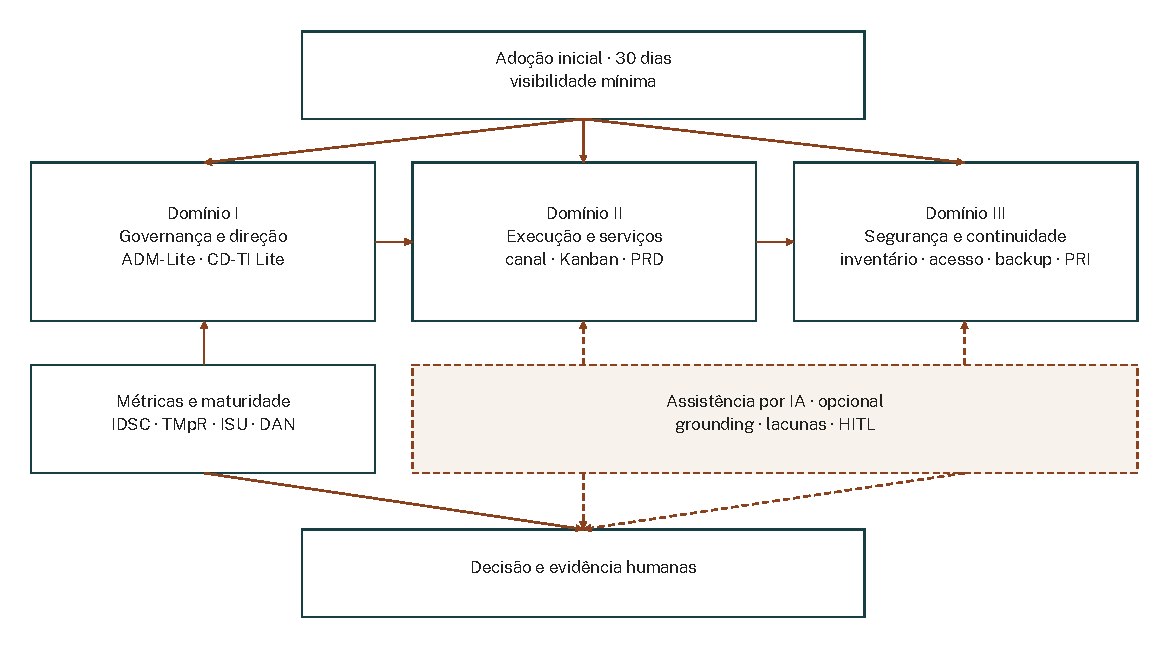
\includegraphics[width=\textwidth]{figures/generated/gppme-architecture.pdf}%
  }{%
    \fbox{\parbox{0.92\textwidth}{\centering
      Fase Zero $\rightarrow$ Governança Essencial $\leftrightarrow$ Execução Ágil $\leftrightarrow$ Segurança Crítica; métricas e maturidade atravessam os três pilares; assistência por IA é opcional e permanece sob HITL.}}
  }
  \caption{Arquitetura conceitual do GP-PME. As setas representam ciclos de informação e decisão, não uma sequência rígida.}
  \label{fig:arquitetura-gppme}
\end{figure}

\subsection{Porta de entrada: diagnóstico e Fase Zero}

O diagnóstico inicial usa dez perguntas binárias, cada resposta positiva condicionada à apresentação de uma evidência. Na versão corrente do artefato, a soma forma o Índice de Maturidade da TI (IM-TI), associado a cinco níveis: 0 (caótico), 1 (organizado reativo), 2 (governança básica), 3 (inovação incremental) e 4 (governança adaptativa). A função do índice é orientar a próxima ação e não certificar conformidade.

A Fase Zero dura 30 dias e estabelece condições mínimas de observação. Na primeira semana, cria-se um canal único de demanda e um quadro Kanban. Na segunda, consolidam-se uma base curta de conhecimento, o inventário de ativos críticos e a situação dos backups. Na terceira, prepara-se um Plano de Resposta a Incidentes (PRI) e inicia-se o CD-TI Lite. Na quarta, publicam-se três indicadores visíveis e o diagnóstico é repetido. Metas sugeridas nesse roteiro são objetivos de desenho; até a execução do protocolo, não constituem resultados médios esperados.

\subsection{Pilar I: Governança Essencial}

O primeiro pilar traduz o ciclo de avaliar, direcionar e monitorar em ADM-Lite. Seu principal ritual é o CD-TI Lite, reunião quinzenal de 30 minutos entre a direção e o responsável por TI. A pauta reserva cinco minutos para indicadores, quinze para alinhamento e priorização, cinco para riscos e dívida técnica e cinco para decisões e responsáveis. A saída é uma ata de uma página, suficiente para registrar o que foi decidido, por quem e com qual evidência de acompanhamento.

A Matriz de Quatro Quadrantes conecta cada iniciativa a uma finalidade de negócio: geração de receita, redução de custos, experiência de cliente ou colaborador, e resiliência ou segurança. O RACI-Lite explicita quem executa, aprova, é consultado e informado, admitindo acumulação de papéis, mas não ausência de responsabilidade. Quando uma iniciativa não encontra vínculo com um quadrante, responsável ou métrica, ela retorna à fila para refinamento.

\subsection{Pilar II: Execução Ágil}

O segundo pilar combina práticas de fluxo e ciclos curtos. Todas as demandas entram por um canal único e percorrem um quadro com quatro estados: A Fazer, Em Andamento, Em Teste e Concluído. O limite padrão de trabalho em progresso é três por executor. O objetivo é tornar filas e bloqueios observáveis, não reproduzir uma implementação integral de Scrum ou ITIL.

A cadência mínima inclui planejamento semanal de quinze minutos, verificação diária de cinco minutos e retrospectiva de quinze minutos. Incidentes críticos usam uma raia de expedite e suspendem explicitamente uma tarefa de menor prioridade, evitando que ``urgente'' signifique trabalho adicional invisível. Demandas de desenvolvimento são reduzidas a um MVP de até duas semanas e documentadas em PRD curto com dor, histórias, critérios verificáveis, escopo negativo, requisito não funcional, métrica afetada e aprovação humana.

\subsection{Pilar III: Segurança Crítica}

O terceiro pilar seleciona controles de maior efeito operacional imediato. O Inventário 80/20 registra os ativos cuja indisponibilidade ou comprometimento afeta a maior parte da operação. Identidade e acesso são tratados por contas individuais, autenticação multifator em sistemas críticos e privilégio mínimo. Backups devem ser automáticos e acompanhados de teste periódico de restauração. O PRI de uma página define contenção, comunicação, responsáveis e recuperação.

Um checklist de dez controles amplia essa linha de base conforme a organização amadurece. Cada item recebe estado (implementado, em andamento ou não implementado), evidência, próximo passo, responsável e prazo. A classificação de risco usa probabilidade e impacto em categorias ordinais; quando faltam dados técnicos, o artefato exige registro da lacuna ou auditoria local, em vez de inferência automática.

\subsection{Métricas transversais}

Três indicadores formam o painel operacional inicial. O Índice de Disponibilidade de Serviços Críticos (IDSC) é dado por
\begin{equation}
  \mathrm{IDSC}=\frac{T_{\text{previsto}}-T_{\text{indisponível}}}{T_{\text{previsto}}}\times 100.
\end{equation}
O Tempo Médio para Resolução (TMpR) é a soma das durações dos chamados encerrados dividida pela quantidade de chamados. O Índice de Satisfação do Usuário (ISU) é a média das notas coletadas no período. Os três valores são discutidos em conjunto, pois disponibilidade alta pode coexistir com resolução lenta ou experiência ruim.

Para decisões de modernização, a Dívida de Arquitetura Normalizada (DAN) relaciona o esforço estimado de refatoração ao orçamento anual de TI:
\begin{equation}
  \mathrm{DAN}=\frac{H_{\text{refatoração}}\times C_{\text{hora}}}{O_{\text{TI, anual}}}.
\end{equation}
O Custo de Oportunidade Tecnológica (COT) consolida custos diretos e indiretos de uma mudança, e o retorno projetado é calculado a partir de premissas registradas. DAN, COT e ROI são instrumentos de decisão e análise de sensibilidade; valores produzidos por cenários não devem ser tratados como retorno observado.

\subsection{Camada opcional de assistência por IA}

A IA é uma camada transversal e opcional. No modo manual, todos os rituais e artefatos podem ser executados com reunião, planilha, quadro e templates. No modo assistido, agentes especializados ajudam a fazer triagem, gerar uma primeira minuta, calcular métricas, recuperar trechos da base de conhecimento e auditar requisitos. A decisão de priorizar, aprovar, alterar acesso, conter incidente ou investir permanece com uma pessoa identificada.

O protocolo de segurança epistêmica possui quatro regras. A saída deve estar ancorada em dados fornecidos ou em fonte recuperada; informações ausentes recebem o marcador de dado insuficiente; cálculos determinísticos são separados de narrativa gerada; e qualquer artefato com efeito organizacional passa por Human-in-the-Loop (HITL). Essa arquitetura procura capturar benefícios de assistência sem converter fluência textual em autoridade decisória.

\subsection{Instanciação computacional}

A versão analisada no repositório \citep{gppme2026repo} instancia o artefato em guias, templates, oito skills, nove agentes prontos, um orquestrador com oito especialistas, cinco adaptadores de plataformas de trabalho, busca textual/semântica, grafo de conhecimento e serviços de API/MCP. Regras como IM-TI, indicadores, DAN, COT e ROI também possuem implementações determinísticas. Esses componentes ampliam os canais de uso do mesmo núcleo de conhecimento; não adicionam novos pilares conceituais.

Alguns documentos históricos chamam a assistência por IA de ``Pilar IV''. Para manter coerência com a hipótese original e com o requisito de funcionamento manual, este artigo adota a nomenclatura ``três pilares essenciais mais uma camada opcional''. A diferença é semântica e arquitetural: uma prática opcional não pode ser condição para que o núcleo do framework seja considerado completo.

\section{Estado documental e alcance da evidência}
\label{sec:estado}

A edição GEAR de outubro consolida o acervo em núcleo, adoção, guias, indicadores, exemplos, modelos, fundamentos e fontes. O \href{https://github.com/andrecodexvictor/GP-Pme/tree/8386586af110ba2112694a8ee6dd7b9d94d20572/framework}{núcleo documental versionado} permite inspecionar a especificação \citep{gppme2026repo}; o \href{https://github.com/andrecodexvictor/GP-Pme/tree/codex/gear-editorial/framework/publicacao}{registro de publicação} identifica o tratamento editorial e seus limites. Fontes externas, adaptações locais e exemplos ilustrativos têm funções distintas na argumentação.

A produção assistida e a auditoria são relatadas a partir desses documentos, da declaração de uso de IA e das correções registradas. A evidência permite examinar coerência e proveniência, mas não estabelecer a contribuição causal de cada ferramenta. Não há resultados de aplicação do GEAR em empresas, de prova de conceito no FrameSim ou de comparação com alternativas. Verificações de software do repositório não são usadas como validação do framework neste artigo.

\section{Protocolo prospectivo de prova de conceito}
\label{sec:protocolo}

\subsection{Perguntas e hipóteses de avaliação}

A prova de conceito futura no FrameSim será guiada por três perguntas. \textbf{PA1}: em empresas simuladas de 5 a 20 colaboradores, qual configuração produz planos mais completos e acionáveis para um conjunto comum de problemas? \textbf{PA2}: qual é o esforço humano e documental exigido para chegar a uma primeira decisão verificável? \textbf{PA3}: em quais condições de porte, maturidade, setor e comportamento das personas cada configuração falha ou exige adaptação?

A hipótese principal é que o GEAR oferece uma relação favorável entre cobertura e esforço nos cenários de baixa maturidade, sem pressupor que supere ITIL~4 ou COBIT~2019 em seus escopos de origem. Duas hipóteses secundárias serão examinadas: os mecanismos relacionais e a Fase Zero terão maior contribuição nos cenários com papéis acumulados; e a camada de IA reduzirá tempo de preparação somente quando contexto, revisão e critérios de saída forem mantidos. Nenhuma dessas hipóteses é tratada como confirmada nesta versão.

\subsection{Desenho pareado dos 25 casos}

Serão executados 25 blocos de teste, cada um correspondente a uma empresa sintética única. Em cada bloco, o mesmo manifesto de empresa, as mesmas personas, os mesmos eventos e o mesmo conjunto de tarefas serão submetidos a três configurações: GEAR, ITIL~4 adaptado e COBIT~2019 adaptado. Assim, 25 testes produzem 75 execuções de framework, mas a unidade de comparação permanece o caso pareado. Os IDs, setores, portes e desafios estão pré-especificados no \cref{ap:casos} e no arquivo suplementar \texttt{scenario-catalog.csv}.

Os casos serão estratificados em cinco faixas de porte (5--7, 8--10, 11--13, 14--16 e 17--20 colaboradores), com cinco empresas por faixa. Setores e incidentes variam para evitar que o resultado dependa de uma única narrativa. A maturidade inicial será limitada aos níveis 0, 1 e 2, coerentes com a porta de entrada do GEAR. Cada caso conterá ao menos uma tensão de direção, uma de fluxo de trabalho e uma de risco, mas sua severidade será balanceada antes das execuções.

\subsection{Configuração justa das alternativas}

A unidade avaliada não será o texto integral de cada referência, mas uma configuração declarada e reproduzível. O GEAR usará sua Fase Zero e seus três domínios essenciais. A configuração ITIL~4 usará princípios orientadores, cadeia de valor e um subconjunto documentado de práticas compatíveis com o pacote de tarefas. A configuração COBIT~2019 usará fatores de desenho e objetivos selecionados por critérios publicados antes do teste. Especialistas deverão revisar os dois baselines para evitar versões deliberadamente fracas.

Como ITIL e COBIT não possuem o mesmo escopo, os resultados serão divididos em dois painéis. O painel de \emph{desempenho no escopo comum} comparará somente tarefas que as três configurações se propõem a tratar. O painel de \emph{cobertura do problema completo} registrará lacunas em direção, serviço e segurança sem interpretar toda ausência como falha intrínseca do framework. Essa decomposição torna visível quando uma diferença decorre do escopo e quando decorre da execução.

No ensaio principal, qualquer assistência por LLM receberá o mesmo modelo, orçamento de contexto, temperatura, ferramentas e tempo entre os três braços. Agentes especializados exclusivos do GEAR não serão usados nessa comparação, pois confundiriam o efeito do conteúdo do framework com o efeito da implementação. A camada opcional de IA será examinada em uma ablação separada, GEAR manual versus GEAR assistido, depois do ensaio principal.

\subsection{Personas mais realistas e reprodutíveis}

Cada empresa terá um núcleo mínimo de quatro funções: proprietário ou direção, responsável por TI (interno ou terceirizado), dono de um processo de negócio e usuário afetado. Em empresas muito pequenas, uma pessoa poderá acumular funções, desde que o manifesto registre o conflito. As demais personas serão sorteadas de um catálogo compatível com setor e porte, sem introduzir cargos incompatíveis com uma equipe de até 20 pessoas.

Uma persona será descrita por cargo, poder decisório, tempo de empresa, disponibilidade semanal para governança, letramento digital, tolerância a risco, abertura à mudança, incentivos, objetivo, conflito, estilo de comunicação e até dois vieses cognitivos. Traços psicológicos não serão usados como diagnóstico clínico. Cada atributo deverá alterar uma regra observável da simulação; atributos puramente ornamentais serão removidos.

As personas do estudo serão sintéticas e não deverão representar indivíduos identificáveis. Antes do congelamento, o catálogo atualmente usado pelo FrameSim deverá passar por revisão de proveniência, licença e conteúdo; qualquer perfil derivado de pessoa real será removido ou transformado em arquétipo anônimo. Essa regra evita que o ganho de realismo seja obtido à custa de privacidade ou consentimento.

A aleatoriedade será hierárquica e registrada. A semente do caso define empresa e evento; a semente de equipe define a seleção e os traços das personas; e a semente de execução controla variações estocásticas. O mesmo manifesto congelado será reutilizado nos três braços. Amostragem aleatória simples será substituída por seleção restrita, verificando cobertura de papéis, soma de colaboradores, compatibilidade setorial, ausência de duplicatas e distribuição de resistência. Esse procedimento preserva diversidade sem perder comparabilidade.

\subsection{Pacote comum de tarefas}

Cada braço deverá responder ao mesmo pacote: (T1) diagnosticar a situação inicial e explicitar dados faltantes; (T2) priorizar cinco demandas concorrentes; (T3) tratar um incidente crítico sem apagar a fila normal; (T4) propor a linha de base de segurança e a evidência de restauração; (T5) transformar uma melhoria em entrega curta com responsável e critério de aceite; e (T6) produzir um painel de decisão com riscos, custos e próximos passos. O conjunto cobre direção, gestão de serviço, execução e segurança, permitindo também identificar lacunas de escopo.

\subsection{Métricas, rubrica e análise}

Os dois desfechos primários serão: \textbf{completude acionável}, pontuada de 0 a 100 por rubrica pré-publicada; e \textbf{esforço humano estimado}, em minutos para compreender, adaptar e aprovar a saída. A rubrica de completude verificará presença de responsável, prazo, entrada, saída, evidência, dependência e critério de encerramento. O esforço será estimado tarefa a tarefa por dois avaliadores e confrontado com número de rituais, papéis obrigatórios e artefatos produzidos.

Os desfechos secundários serão cobertura do pacote, rastreabilidade até fonte ou dado do caso, densidade documental, tempo computacional, custo de tokens, taxa de afirmações sem suporte por 100 afirmações verificáveis, número de correções HITL, violações de restrições, plausibilidade do cenário e aceitação simulada das personas. ``Aceitação simulada'' será reportada como comportamento do modelo, nunca como satisfação de trabalhadores reais.

Dois avaliadores humanos, cegos aos rótulos dos braços quando o conteúdo permitir, aplicarão a rubrica em ordem aleatória. Divergências serão resolvidas por consenso ou terceiro avaliador, e a concordância será reportada. O CriticAgent do FrameSim poderá apontar inconsistências, mas não será o juiz final. Falha do crítico, timeout ou resposta inválida produzirá valor ausente e log de erro; nunca uma nota substituta máxima.

Os resultados serão resumidos por mediana e intervalo interquartil. Diferenças pareadas por caso serão apresentadas com intervalos de confiança bootstrap. Se as premissas forem atendidas, o teste de Friedman examinará diferença global entre os três braços, seguido por comparações de Wilcoxon com correção de Holm e tamanho de efeito. Com 25 casos sintéticos, a análise terá caráter exploratório; valores de $p$ não serão usados para sugerir validade externa.

\begin{table}[htbp]
  \centering
  \caption{Tabela principal reservada para os resultados futuros. Traços indicam dados ainda não coletados.}
  \label{tab:resultados-planejados}
  \small
  \begin{tabular}{@{}lccc@{}}
    \toprule
    Métrica & GEAR & ITIL 4 adaptado & COBIT 2019 adaptado \\
    \midrule
    Completude acionável $\uparrow$ & -- & -- & -- \\
    Esforço humano (min) $\downarrow$ & -- & -- & -- \\
    Rastreabilidade (\%) $\uparrow$ & -- & -- & -- \\
    Afirmações sem suporte/100 $\downarrow$ & -- & -- & -- \\
    Correções HITL $\downarrow$ & -- & -- & -- \\
    \bottomrule
  \end{tabular}
\end{table}

\begin{figure}[H]
  \centering
  \IfFileExists{figures/generated/results-template.pdf}{%
    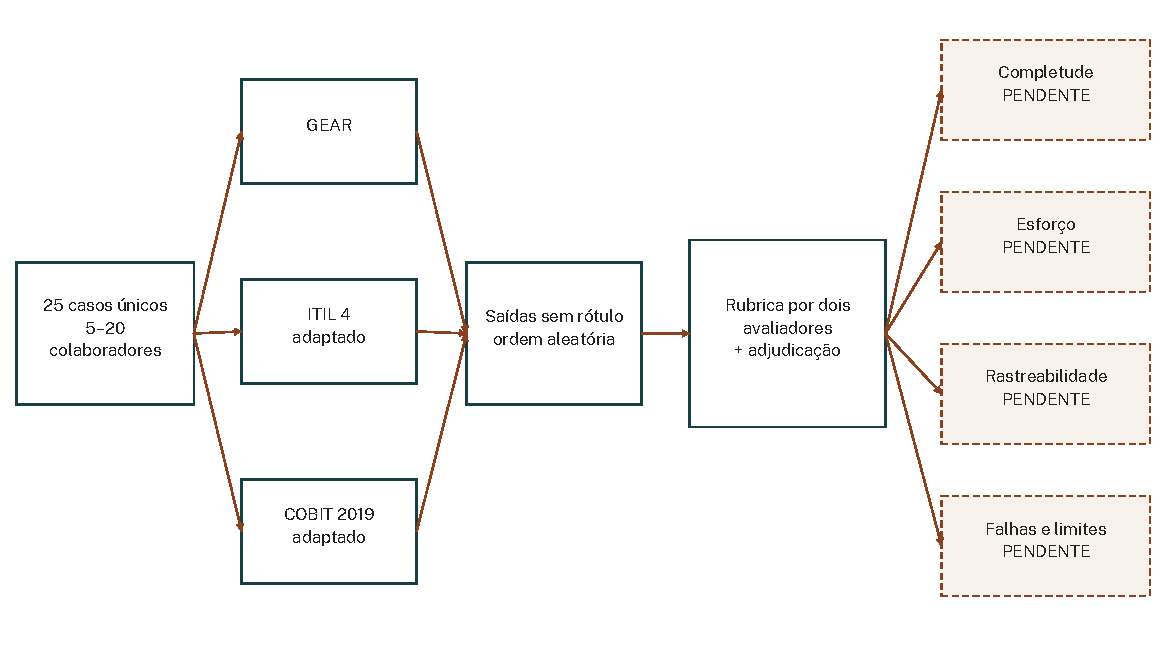
\includegraphics[width=0.95\textwidth]{figures/generated/results-template.pdf}%
  }{%
    \fbox{\parbox{0.88\textwidth}{\centering
      25 casos pareados $\rightarrow$ 3 configurações $\rightarrow$ rubrica cega $\rightarrow$ métricas e falhas $\rightarrow$ síntese comparativa (valores pendentes).}}
  }
  \caption{Modelo Mermaid para a síntese dos resultados. O diagrama representa o protocolo; não contém desempenho observado.}
  \label{fig:resultados-template}
\end{figure}

\subsection{Pré-condições no FrameSim}

O \href{https://github.com/andrecodexvictor/FrameSim}{FrameSim} é o ambiente previsto para a prova de conceito \citep{framesim2026repo}. Antes da coleta, sua versão deverá ser fixada e sua instrumentação conferida quanto a quatro requisitos: aleatoriedade semeada; reutilização de manifestos congelados entre os três braços; registro de erro ou dado ausente quando o avaliador automatizado falhar; e exportação de versões, parâmetros, prompts, fontes recuperadas e erros. São condições de aceitação do protocolo futuro, sem alegação de auditoria atual do código do simulador.

O atendimento e congelamento dessas condições deverá gerar um identificador de protocolo e um \emph{hash} para cada manifesto. Um teste piloto fora dos 25 casos verificará parsing, equilíbrio de tokens, cegamento dos rótulos e cálculo das métricas. O piloto poderá corrigir defeitos de instrumentação, mas não alterar hipóteses ou rubricas após a inspeção dos resultados principais.

\section{Discussão}
\label{sec:discussao}

\subsection{Contribuição teórica e de desenho}

O GEAR sugere que a simplificação de governança não precisa significar remoção arbitrária de controles. Uma alternativa é preservar funções essenciais e reduzir a carga de coordenação por meio de papéis acumuláveis, cadências curtas, artefatos de uma página e evidência mínima. Essa lógica aproxima a teoria da contingência de uma especificação operacional: cada mecanismo deve justificar seu custo pela decisão, risco ou fluxo que torna observável.

O artefato também ajuda a separar governança, gestão e automação. Governança define direção, responsabilidade e monitoramento; gestão organiza o fluxo que transforma direção em serviço; segurança trata riscos que podem comprometer o valor; e IA pode assistir tarefas informacionais sem receber autoridade própria. Essa separação reduz a tendência de apresentar um conjunto de agentes como se fosse, por si só, um modelo de governança.

\subsection{Pesquisa assistida e responsabilidade de conteúdo}

O relato de produção explicita uma distinção necessária ao uso de IA na pesquisa: gerar uma formulação e sustentar uma afirmação exigem operações diferentes. A IA auxiliou a organização e a redação; as fontes consultadas sustentam as afirmações externas, e as decisões autorais identificam adaptações. A auditoria torna visíveis problemas como misturar versões, transferir percentuais de outras tarefas e confundir exemplos com resultados. O registro de uma correção permite examinar a decisão, sem provar que todas as incorreções foram encontradas.

Esse procedimento pode orientar outras pesquisas de desenho que usem IA, mas sua transferência permanece uma proposta metodológica. O trabalho não compara produção manual e assistida, não estima precisão da IA e não demonstra que a auditoria tenha uma taxa de detecção superior. O histórico incompleto de interações, o envolvimento do autor no desenho e na revisão e o acesso parcial a algumas fontes limitam a reprodutibilidade e a independência do relato. Uma avaliação posterior desse processo precisaria de corpus fixo, registros completos e revisores independentes.

\subsection{Implicações práticas}

Para uma empresa pequena, a porta de entrada importa tanto quanto o catálogo de boas práticas. Começar por canal, quadro, inventário, backup, resposta a incidente e reunião curta cria dados que antes não existiam e permite que decisões posteriores sejam menos intuitivas. A Fase Zero é, portanto, uma hipótese de sequência: visibilidade operacional antecede sofisticação de processo.

Para consultores e responsáveis de TI, a rastreabilidade até referências de origem define o limite do termo ``Lite''. O GEAR pode indicar uma linha de base e produzir evidências iniciais, mas não deve prometer certificação ISO, conformidade integral com NIST/CIS, ou implantação completa de ITIL e COBIT. Quando regulação, criticidade ou porte excederem o recorte, o resultado correto do diagnóstico é escalar a análise para especialista e estrutura apropriados.

\subsection{Melhorias de desenho identificadas}

A edição de outubro desacoplou maturidade central de adoção de IA. O questionário histórico incluía uso de IA com HITL na pontuação global, embora a IA fosse declarada opcional. As dez perguntas correntes verificam práticas de governança, execução, segurança e medição, permitindo alcançar o nível máximo sem IA. Resultados históricos exigem reaplicação antes de comparação. Se a organização considerar assistência por IA, deverá avaliar separadamente dados, validação, rastreabilidade e supervisão; essa análise não altera o IM-TI nem constitui uma nova escala validada.

A segunda melhoria é publicar uma matriz normativa por prática. Cada controle do GEAR deverá apontar para sua fonte, versão, objetivo, grau de cobertura e evidência exigida. Essa matriz reduzirá ambiguidades como chamar um checklist interno de ``NIST-Lite'' e permitirá atualizar o artefato quando uma norma mudar, sem reescrever todo o modelo.

A terceira melhoria é tornar metas e fórmulas sensíveis ao contexto. Limiares de disponibilidade, tempo de resolução, satisfação, DAN e payback são úteis como valores iniciais, mas não podem ser universais. O diagnóstico deve registrar janela de observação, criticidade do serviço, custo-hora, sazonalidade e qualidade da fonte. A comparação futura também deverá apresentar análise de sensibilidade, em vez de um ROI pontual.

A consolidação terminológica fixa três domínios essenciais e assistência por IA opcional. Essa escolha evita que o nome GEAR ou as quatro letras sejam interpretados como quatro pilares. A versão documental, suas fontes e as regras de leitura devem permanecer identificáveis a cada revisão.

\subsection{Ameaças à validade}

A validade de constructo é limitada pela mensuração de conceitos como ``acionabilidade'', ``overhead'' e ``aceitação''. Rubricas publicadas, dupla avaliação e apresentação das métricas componentes reduzem o risco de que um índice composto esconda trade-offs. Reações de personas e plausibilidade do crítico continuarão sendo propriedades da simulação, não medidas de comportamento humano real.

A validade interna pode ser afetada pelo modelo de linguagem, ordem dos prompts, recuperação documental, aleatoriedade e conhecimento prévio do avaliador. O protocolo prevê controlar esses fatores com manifestos pareados, sementes, orçamento equivalente, rótulos embaralhados, logs completos e tratamento explícito de falhas. Ainda assim, uma saída pode favorecer padrões com maior presença nos dados de treinamento do modelo.

A validade externa é a principal limitação. Os 25 casos cobrem somente organizações sintéticas de 5 a 20 colaboradores, com cenários inspirados em pequenas empresas brasileiras. Setores regulados aparecem como testes de estresse, não como autorização de uso profissional. Mesmo um resultado consistente no FrameSim sustentará apenas uma prova de conceito dentro do simulador; generalização requer implantação longitudinal em empresas reais.

A validade de conclusão também será restrita pela amostra de 25 casos e pela multiplicidade de métricas. O estudo priorizará estimativas pareadas, intervalos e falhas observadas, usando testes de hipótese apenas como apoio exploratório. Resultados nulos ou desfavoráveis serão mantidos e deverão orientar revisão do artefato.

\subsection{Agenda de avaliação}

O próximo ciclo possui três etapas. Primeiro, verificar a prontidão e fixar a instrumentação do FrameSim e registrar o protocolo antes de observar os resultados. Segundo, executar o piloto e os 25 casos pareados, publicar os manifestos, saídas anonimizadas, rubricas e scripts de análise. Terceiro, selecionar casos contrastantes para estudo de campo, acompanhando tempo de adoção, aderência às rotinas, incidentes, qualidade decisória e abandono de práticas ao longo de meses.

Uma avaliação posterior deverá ainda isolar os componentes do GEAR. Remover a Fase Zero, o limite de WIP, o CD-TI Lite, a linha de base de segurança ou a camada de IA permitirá investigar qual mecanismo produz cada mudança e em que contexto. Sem essa ablação, um eventual ganho do pacote completo não explica sua causalidade.

\section{Conclusão}
\label{sec:conclusao}

O GEAR organiza uma proposta de governança e gestão de TI para pequenas equipes em três domínios essenciais, um percurso inicial de 30 dias, indicadores e modelos compactos. A construção combina leitura dirigida de referências, síntese e adaptações autorais, com assistência por IA na pesquisa e na produção. O artigo explicita o procedimento de auditoria de conteúdo usado para conferir fontes, preservar limites e corrigir inconsistências.

As contribuições atuais são a especificação documental do framework e o relato rastreável dessa produção assistida. O uso de IA não fornece evidência de eficácia do GEAR, e os registros editoriais não permitem estimar um benefício causal da própria assistência. A ausência de uma revisão sistemática exaustiva, o acesso parcial a algumas fontes e o histórico incompleto de interações delimitam o alcance do relato.

A avaliação do framework permanece futura. O protocolo prevê uma prova de conceito no FrameSim com 25 empresas sintéticas, três configurações pareadas, tarefas comuns e critérios previamente definidos. Nenhuma rodada foi realizada nesta versão e nenhuma tabela contém resultados observados. A prova de conceito poderá revelar cobertura, esforço estimado e falhas nos cenários; evidência de aprendizagem, adesão e efeito organizacional exigirá estudos posteriores em empresas reais.


\section*{Declaração de uso de inteligência artificial}
Ferramentas de IA generativa foram usadas ativamente na leitura assistida do acervo, na elaboração de sínteses e minutas, na comparação entre versões, na identificação de inconsistências e na preparação editorial de texto, LaTeX e diagramas. A revisão incluiu conferência de fontes e correções de conteúdo, descritas na \cref{sec:auditoria-ia}. Saídas de IA não foram tratadas como fontes bibliográficas ou dados empíricos. O autor responde pela seleção, interpretação e versão final. Não se dispõe de um registro uniforme de modelos, prompts e intervenções de toda a produção histórica; o relato não equivale a uma avaliação experimental da IA. Nenhuma rodada comparativa do FrameSim foi executada.

\section*{Disponibilidade de artefatos}
O \href{https://github.com/andrecodexvictor/GP-Pme/tree/codex/gear-editorial}{repositório GEAR, branch editorial}, reúne o núcleo documental, as fontes deste artigo, diagramas e catálogo prospectivo de cenários. A \href{https://github.com/andrecodexvictor/GP-Pme/tree/8386586af110ba2112694a8ee6dd7b9d94d20572}{revisão editorial de referência} fixa o estado anterior a esta atualização; o registro de publicação identifica as revisões seguintes. O \href{https://github.com/andrecodexvictor/Frame-sim}{FrameSim} será o ambiente da prova de conceito. Logs e resultados dependerão do congelamento e da execução futura do protocolo, com distribuição nos termos das licenças aplicáveis.

\section*{Aspectos éticos}
Esta versão não envolve participantes humanos nem coleta de dados organizacionais. A avaliação planejada empregará empresas e personas sintéticas sem identificação de pessoas reais. Estudos de campo posteriores dependerão de consentimento, proteção de dados e apreciação ética institucional quando aplicável.

\section*{Agradecimentos}
O projeto de pesquisa que originou este trabalho foi desenvolvido no IFBA, Campus Vitória da Conquista, sob orientação da Profa. Dra. Viviane Maria Lélis Carvalho e coorientação do Prof. Dr. Crescencio Rodrigues Lima Neto. A inclusão de nomes nesta seção não implica coautoria; a autoria final deverá ser confirmada antes da submissão.

\bibliographystyle{plainnat}
\bibliography{references}

\clearpage
\appendix
\section{Catálogo pré-especificado dos 25 casos}
\label{ap:casos}

\begingroup
\footnotesize
\renewcommand{\arraystretch}{1.08}
\setlength{\tabcolsep}{4pt}
\begin{longtable}{@{}L{0.8cm}L{2.8cm}L{1.0cm}L{1.0cm}L{7.0cm}@{}}
  \caption{Empresas sintéticas planejadas. O nível indica a maturidade inicial (0--2).}\label{tab:catalogo-casos}\\
  \toprule
  ID & Setor & Colab. & Nível & Desafio principal \\
  \midrule
  \endfirsthead
  \toprule
  ID & Setor & Colab. & Nível & Desafio principal \\
  \midrule
  \endhead
  C01 & Contabilidade & 5 & 0 & Senhas compartilhadas, phishing e fechamento mensal dependente de uma estação. \\
  C02 & Comércio eletrônico & 6 & 1 & Pedidos dispersos entre marketplace e mensagens; prioridades mudam diariamente. \\
  C03 & Clínica odontológica & 7 & 1 & Agenda instável, dados pessoais e ausência de teste de restauração. \\
  C04 & Construção civil & 7 & 0 & Arquivos de obra em dispositivos locais e decisões técnicas sem responsável claro. \\
  C05 & Alimentação e delivery & 6 & 1 & Queda do ponto de venda durante o pico e atendimento por canais paralelos. \\
  C06 & Curso profissionalizante & 8 & 1 & Matrículas manuais, base duplicada e suporte sem fila visível. \\
  C07 & Hospedagem & 9 & 1 & Reservas em canais distintos, acesso compartilhado e conflito entre recepção e direção. \\
  C08 & Advocacia & 10 & 0 & Documentos sensíveis sem classificação e fornecedor de TI sem acordo de responsabilidades. \\
  C09 & Autopeças & 10 & 2 & Estoque e ERP divergentes, backlog de integrações e indisponibilidade recorrente. \\
  C10 & Logística local & 9 & 1 & Operação coordenada por mensagens pessoais e falha de rastreio de entregas. \\
  C11 & Confecção & 11 & 0 & Planejamento em planilhas isoladas e máquina crítica sem inventário de dependências. \\
  C12 & Farmácia & 12 & 1 & Risco de ransomware, estoque regulado e recuperação nunca exercitada. \\
  C13 & Arquitetura & 13 & 2 & Equipe híbrida, versões conflitantes de projetos e dívida de armazenamento. \\
  C14 & Software como serviço & 12 & 2 & Backlog excessivo, incidente de acesso e pressão por lançar em duas semanas. \\
  C15 & Serviços agrícolas & 11 & 1 & Suporte de campo intermitente, equipamento compartilhado e baixa conectividade. \\
  \pagebreak
  C16 & Restaurante (duas unidades) & 14 & 1 & Pontos de venda heterogêneos e decisão sobre consolidação com orçamento restrito. \\
  C17 & Laboratório clínico & 15 & 2 & Dados sensíveis, cadeia de backup incompleta e dependência de fornecedor externo. \\
  C18 & Agência de marketing & 16 & 1 & Ferramentas contratadas sem aprovação, retrabalho e permissões não revogadas. \\
  C19 & Atacado & 15 & 2 & Integração fiscal/ERP legada, fila de mudanças e disputa entre custo e continuidade. \\
  C20 & Assistência técnica & 14 & 1 & Chamados sem SLA, peças sem vínculo com ordens e escaladas informais. \\
  C21 & Panificação industrial & 17 & 1 & Rastreabilidade de lote, terminais antigos e manutenção reativa. \\
  C22 & Pequena rede hoteleira & 18 & 2 & Três unidades, perfis de acesso inconsistentes e indicadores não consolidados. \\
  C23 & Edtech & 20 & 2 & Incidente em período de prova, dívida técnica e pressão simultânea por novas funções. \\
  C24 & Organização social & 19 & 1 & Dados de doadores, equipe voluntária e governança de fornecedores em nuvem. \\
  C25 & Metalurgia & 20 & 0 & Dependência de computador de produção, ausência de inventário e decisão centralizada no dono. \\
  \bottomrule
\end{longtable}

Cada descrição será expandida por um manifesto JSON versionado contendo premissas econômicas, stack tecnológica, eventos, tarefas, critérios de sucesso, personas, papéis acumulados e sementes. A narrativa pode variar dentro dessas restrições, mas setor, porte, nível e desafio principal permanecerão congelados entre os braços.
\endgroup


\end{document}
